\documentclass[a4paper]{article}
\usepackage{fancyhdr}
\usepackage{enumitem}
\usepackage{tikz}

\title{Homework module: Compiler Technology}

\lhead{Homework module \#2}
\rhead{TDT4205 - Compilers}

\author{Aleksander Vognild Burkow}

\begin{document}

\maketitle
\thispagestyle{empty}
\newpage

\part{Theory}
\section{Regular languages}

\begin{enumerate}[label=\alph*)]
\item Convert the regular expression $ a(b|c)d\*e $ to a NFA.

\begin{figure}[H]
\begin{center}
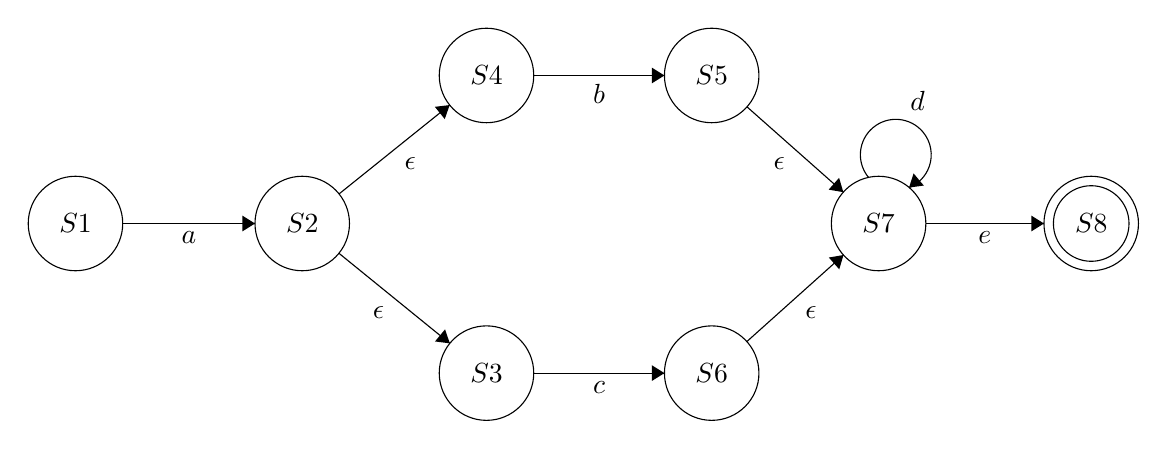
\begin{tikzpicture}[scale=0.2]
\tikzstyle{every node}+=[inner sep=0pt]
\draw [black] (8.1,-31) circle (3);
\draw (8.1,-31) node {$S1$};
\draw [black] (22.5,-31) circle (3);
\draw (22.5,-31) node {$S2$};
\draw [black] (34.2,-40.5) circle (3);
\draw (34.2,-40.5) node {$S3$};
\draw [black] (34.2,-21.6) circle (3);
\draw (34.2,-21.6) node {$S4$};
\draw [black] (48.5,-21.6) circle (3);
\draw (48.5,-21.6) node {$S5$};
\draw [black] (48.5,-40.5) circle (3);
\draw (48.5,-40.5) node {$S6$};
\draw [black] (59.1,-31) circle (3);
\draw (59.1,-31) node {$S7$};
\draw [black] (72.6,-31) circle (3);
\draw (72.6,-31) node {$S8$};
\draw [black] (72.6,-31) circle (2.4);
\draw [black] (11.1,-31) -- (19.5,-31);
\fill [black] (19.5,-31) -- (18.7,-30.5) -- (18.7,-31.5);
\draw (15.3,-31.5) node [below] {$a$};
\draw [black] (24.84,-29.12) -- (31.86,-23.48);
\fill [black] (31.86,-23.48) -- (30.92,-23.59) -- (31.55,-24.37);
\draw (29.36,-26.79) node [below] {$\epsilon$};
\draw [black] (24.83,-32.89) -- (31.87,-38.61);
\fill [black] (31.87,-38.61) -- (31.57,-37.72) -- (30.93,-38.49);
\draw (27.34,-36.24) node [below] {$\epsilon$};
\draw [black] (37.2,-40.5) -- (45.5,-40.5);
\fill [black] (45.5,-40.5) -- (44.7,-40) -- (44.7,-41);
\draw (41.35,-41) node [below] {$c$};
\draw [black] (37.2,-21.6) -- (45.5,-21.6);
\fill [black] (45.5,-21.6) -- (44.7,-21.1) -- (44.7,-22.1);
\draw (41.35,-22.1) node [below] {$b$};
\draw [black] (50.74,-23.59) -- (56.86,-29.01);
\fill [black] (56.86,-29.01) -- (56.59,-28.1) -- (55.93,-28.85);
\draw (52.79,-26.79) node [below] {$\epsilon$};
\draw [black] (58.467,-28.08) arc (219.96376:-68.03624:2.25);
\draw (61.57,-23.87) node [above] {$d$};
\fill [black] (61.03,-28.72) -- (61.97,-28.59) -- (61.32,-27.82);
\draw [black] (62.1,-31) -- (69.6,-31);
\fill [black] (69.6,-31) -- (68.8,-30.5) -- (68.8,-31.5);
\draw (65.85,-31.5) node [below] {$e$};
\draw [black] (50.73,-38.5) -- (56.87,-33);
\fill [black] (56.87,-33) -- (55.94,-33.16) -- (56.6,-33.91);
\draw (54.81,-36.24) node [below] {$\epsilon$};
\end{tikzpicture}
\caption{NFA}
\label{fig:nfa}
\end{center}
\end{figure}


\end{enumerate}


\end{document}
